% !TEX program = XeLaTeX
% !TEX encoding = UTF-8
\documentclass[UTF8,nofonts]{article}
%{ctexart}


%\setCJKmainfont[BoldFont=FandolSong-Bold.otf,ItalicFont=FandolKai-Regular.otf]{FandolSong-Regular.otf}
%\setCJKsansfont[BoldFont=FandolHei-Bold.otf]{FandolHei-Regular.otf}
%\setCJKmonofont{FandolFang-Regular.otf}

\usepackage{url}
\usepackage{cancel}
\usepackage{xspace}
\usepackage{graphicx}
\usepackage{multicol}
\usepackage{multirow}
\usepackage{subfig}
\usepackage{amsmath}
\usepackage{amssymb}
%\usepackage[a4paper, width=180mm, top=18mm, bottom=22mm, includeheadfoot]{geometry}
\usepackage[a4paper, width=140mm, top=18mm, bottom=22mm, includeheadfoot]{geometry}
\usepackage{booktabs}
\usepackage{array}
\usepackage{verbatim}
\usepackage{caption}
%\usepackage{natbib}
\usepackage{booktabs}
\usepackage{float}
\usepackage{pdflscape}
\usepackage{mathtools}
\usepackage[usenames, dvipsnames]{xcolor}
\usepackage{afterpage}
\usepackage{pgf}
\usepackage{tikz}
\usepackage{dirtree}
\usepackage{amsfonts}
\usepackage{tkz-graph}


\newtheorem{definition}{Definition}[section]
\newtheorem{theorem}{Theorem}[section]
\newtheorem{lemma}{Lemma}
\newtheorem{proof}{Proof} [section]



\usepackage[toc, page, title, titletoc, header]{appendix}
\usepackage{marginnote}
\usepackage{tablefootnote}

%\renewcommand\appendixname{附\ 录}
%\renewcommand\appendixpagename{附\ 录}
%\renewcommand\appendixtocname{附\ 录}
\renewcommand\abstractname{Abstract}


\usepackage{perpage} %the perpage package
\MakePerPage{footnote} %the perpage package command

\usetikzlibrary{shapes.geometric}%
\usepackage{color}
%\usepackage[pages=some, placement=top]{background}
\usepackage{eso-pic}

\title{Multilateral Token Trade Protocol (MTTP)\\v0.8}
\author{
  daniel@mttp.io\\
  jay@mttp.io\\
  alex@mttp.io\\ 
  \\
  \textit{MTTP Foundation}\\
  \textit{http://mttp.io}\\
  \textit{foundation@mttp.io}\\
 }

\makeatletter
\def\CTEX@section@format{\Large\bfseries}
\makeatother

\makeatletter
\newenvironment{tablehere}
 {\def\@captype{table}}
 {}

\newenvironment{figurehere}
 {\def\@captype{figure}}
 {}
\makeatother

\newcommand\BackgroundPic{%
\put(0, 0){%
\parbox[b][\paperheight]{\paperwidth}{%
\vfill
\centering

\includegraphics[width=\paperwidth, height=\paperheight, %
%keepaspectratio]{images/background.jpg}%
]{images/background.jpg}%
\vfill
}}}


\begin{document}
\AddToShipoutPicture{\BackgroundPic}
\maketitle
This document is for informational purposes only and does not constitute an offer or solicitation to sell shares or securities. Any such offer or solicitation will be made only by means of a confidential offering memorandum and in accordance with the terms of all applicable securities and other laws.



\begin{abstract}
Multilateral token exchange protocol (MTTP) is an open protocol for decentralized exchange on the Ethereum blockchain. MTTP is intended to serve as an open standard and common building block,  driving interoperability among decentralized applications (DAPPs) that incorporate exchange functionality. Trades are executed by a system of Ethereum smart contracts that are publicly accessible,  free to use, and that any dApp can hook into.
\end{abstract}

\newpage

\tableofcontents
\newpage

\section{Background\label{sec: background}}

Blockchain\cite{staff2016blockchains}\cite{swan2015blockchain} technology was created to facilitate the cryptocurrency Bitcoin\cite{nakamoto2008Bitcoin}. It is originally a decentralized system to enforce the financial agreements\cite{lamport1982byzantine}\cite{christidis2016blockchains}. The technology that underlies them could spread into other transactions: trading stock,  IP, buying and selling real estate, purchasing music and much more. Both consortium blockchain and private blockchain have been developed and implemented during the last few years, the value, however, only exists among the closed set of entities or internal entity. While fully public blockchain operates by having a large number of participants,  resulting in trust by numbers. According to coinmarketcap.com stats,  the total cryptocurrency market cap value has reached to 113 billions USD,  including 32 billions USD from Ethereum\cite{wood2014ethereum} on June 12, 2017.

Blockchain has massive influence on the many areas,  particular in finance industry. It is strongly believed that tokenization\cite{liu2016medical}\cite{christidis2016blockchains}\cite{swan2015blockchain} is a new solution. Asset tokenization can reduce the cost,  globalize the asset and increase the liquidation. We will see more dApps that require the use of these different tokens. As a result,  an open standard for exchanging tokens is critical to support this open economy.

A regular exchange platform is based on peer-to-peer IOUs and blockchain technology. Firstly,  users need to deposit their money or tokens into exchange's  bank account or wallet,  then their account will be credited some IOU. Thus,  users actually are trading their IOU in the exchange. Users have to file a ticket when they want to withdraw or sell the tokens.

In February 2014,  the largest Bitcoin exchange "Mt. Gox" suspended trading,  closed its website and exchange service,  and filed for bankruptcy protection from creditors\cite{mcmillan2014inside}. Mt. Gox announced that approximately 850,000 Bitcoins belonging to customers and the company were missing and likely stolen,  an amount valued at more than \$450 million at the time. Research showed less than 1 percent (7000 btc) of missing funds lost to attacks. In 2016,  Bitfinex was the subject of the Bitfinex Hack, in which \$72 million in Bitcoin was stolen from the company's customer's accounts. Therefore,  lack of regulation is hurting Bitcoin in many regions. It also approves that the centralized exchange platform has those unavoidable risk.

We describe a protocol that facilitates decentralized exchange mechanism of ERC20 tokens on the Ethereum blockchain to solve above issues. One of the strength for decentralization is not holding by any party,  thus asset-stealing becomes impossible, which can build up the trust between customers and exchange at a very low cost. In addition, this mechanism has no time and region limits, is highly transparent and has traceable features. All those features make transactions more liquidatable and minimize the price spread.

\section{Market and Industry\label{sec: existingworks}}

There are some decentralized exchanges on blockchain technology like Ripple,  BitShares,  Openledger in open sourced community.

Ripple\cite{schwartz2014ripple} is a real-time gross settlement system,  currency exchange and remittance network operated by Ripple (the company). Also called the Ripple Transaction Protocol (RTXP) or Ripple protocol,  it is built upon a distributed open source Internet protocol,  consensus ledger. Ripple's solution is built around an open,  neutral protocol (Interledger Protocol or ILP\cite{thomas2015protocol}) to power payments across different ledgers and networks globally. It offers a cryptographically secure end-to-end payment flow with transaction immutability and information redundancy. Architected to fit within a bank's existing infrastructure,  Ripple is designed to comply with risk,  privacy and compliance requirements.

BitShares\cite{schuhbitshares}\cite{schuh2015bitshares} is an industrial-grade financial blockchain smart contracts platform. The BitShares decentralized exchange - also known as "The DEX" is a next-generation cryptocurrency trading platform. The DEX is inherently decentralized,  enabling you to trade the BitShares core token (BTS) and a range of trust-less price-stable,  market-pegged assets such as bitUSD,  bitCNY,  bitBTC,  bitGold and more. These assets can all be traded with zero counter-party risk,  putting you in total control of your funds. However,  Bitshares project has many limitations on itself.

The OpenLedger Dex\cite{openledger} is a cryptocurrency exchange. It allows users to exchange Bitcoin into SmartCoins and then withdraw the smartcoins and convert them into cash through PayPal,  Ripple or NanoCard. Additionally,  openledger highly relies on BitShares 2.0 platform and Graphene Toolkit's operation.

The Bancor\cite{bancor}\cite{hanson2012logarithmic} protocol enables built-in price discovery and a liquidity mechanism for tokens on smart contract blockchains. These "smart tokens" hold one or more other tokens in reserve and enable any party to instantly purchase or liquidate the smart token in exchange for any of its reserve tokens,  directly through the smart token's contract,  at a continuously calculated price, according to a formula which balances buy and sell volumes.

"0x"\cite{warren20170x} is a protocol that facilitates low friction peer-to-peer exchange of ERC20\cite{ERC20} tokens on the Ethereum blockchain. The protocol is intended to serve as an open standard and common building block,  driving interoperability among decentralized applications (dApps) that incorporate exchange functionality. Trades are executed by a system of Ethereum smart contracts that are publicly accessible,  free to use and that any dApp can hook into. DApps built on top of the protocol can access public liquidity pools or create their own liquidity pool and charge transaction fees on the resulting volume. While,  0x protocol has many limitations including,  only accept simple OTC order; unclear competing mechanism among each exchanges; lack of protection mechanism for miners.

Due to above reasons and limitation,  centralized exchange is now still playing an important role in cryptocurrency market. Nevertheless,  Our team has inspired by both 0x protocol and payment channel and brought up a new solution for decentralized exchange protocol.


\section{Design Protocol\label{sec: protocol}}

\begin{center}
\begin{figurehere}
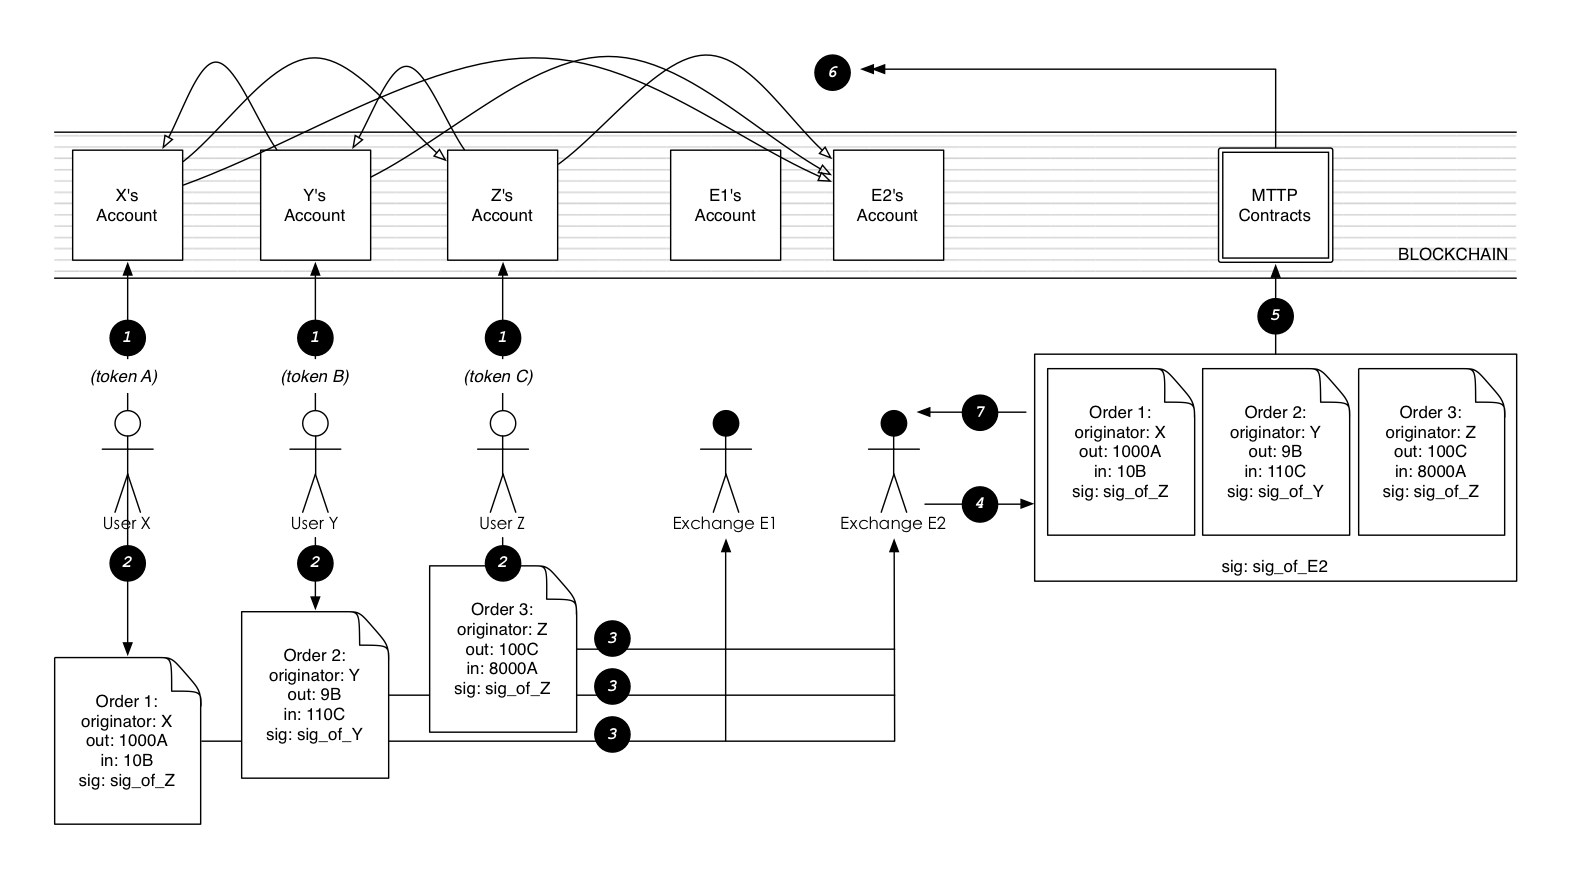
\includegraphics[height=8cm]{images/en_protocol.png}
\caption{Figure shows mix and match 3 orders}
\label{fig: MTTProtocol}
\end{figurehere}
\end{center}

Figure 1 presents the general sequence of steps used for three parties transaction under MTTP:

\begin{enumerate}
 \item User X,  Y and Z authorize MTTP smart contract to manipulate their accounts for token trading and exchanging. From above figure,  Contract may transfer out 1000 token A from User X's account,  and transfer out 9 token B from User Y's account,  100 token C from User Z's account;
 \item User X,  Y and Z place their own orders with signature using their private keys. Thus,  all the orders go into a medium and ready to exchange - Order 1 is selling no more than 1000 token A and purchase no less than 10 token B; if the order is partially matched,  then exchange rate between A to B should be no less than 1000/10=100.00 (Selling tokens divided by purchasing tokens). We will illustrate other involved parameters in chapter 3.7;
 \item User X,  Y and Z continue to send their order to one of the other multiple exchanges;
 \item After the exchange received three separated orders,  they will replace them into corresponding order-book, while update new block and calculate each order's status in order to match the set order - since we call it ring exchange or matching exchange. Once all the orders are confirmed and successfully mix-matched;
 \item Exchange will send out a signature to MTTP smart contract address;
 \item MTTP smart contract will verify quadruple signatures in order to verify three orders' closing. If closing is failed,  then terminate the contract (exchange still cost certain gas); otherwise,  smart contract needs to calculate the proceed and cost for each users, then complete the token exchange. During each steps, MTTP smart contract will use MTTP Registration Contract to calculate all the fees and discount before closing,  system will also need to use MTTP Stats Contract to update database.
 \item Exchange starts receiving new block and new data from the chain in order to upgrade the order-book then to mix-match new and existing orders.
\end{enumerate}


\subsection{Definition of Symbol}

First we would introduce the definition of each symbol.
\[
\begin{split}
&C_{i}\text{: \ }\text{stands for the $i$-th token.}\\
&O_{i\rightarrow j}\text{: \ }\text{stands for an order selling token $C_{i}$ for token $C_{j}$ .}\\
&s_{i\rightarrow j}\text{: \ }\text{selling token upper limit in order $O_{i\rightarrow j}$.}\\
&b_{i\rightarrow j}\text{: \ }\text{buying token lower limit in order $O_{i\rightarrow j}$.}\\
&r_{i\rightarrow j}\text{: \ }\text{max exchange rate in order $O_{i\rightarrow j}$, which is $s_{i\rightarrow j} / b_{i\rightarrow j}$.}
\end{split}
\]ring


We underlined the symbols to emphasis on their original numbers. For example $\overline{s}_{i\rightarrow j}$ and $\overline{b}_{i\rightarrow j}$ stands for number of token from the original order

\subsection{Rate Immutability\label{sec: consistrate}}

MTTP demands the max-return exchange rate in an order stay immutable until the order is closed: 
$s_{i\rightarrow j} / b_{i\rightarrow j} = \overline{s}_{i\rightarrow j}/ \overline{b}_{i\rightarrow j}$. This guarantees after an order is partially filled, the remaining order still satisfies the user's original intention.

\subsection{Order Reducibility\label{sec: reducibility}}


We can use token $C_j$ to connect two orders ( $O_{i\rightarrow j}$ and $O_{j\rightarrow k}$ ),  regard it as one single order for selling token $Ci$ for buying token $C_k$. we use $O_{i\rightarrow j\rightarrow k}$ to represent this order. This order $O_{i\rightarrow k}$'s properties can be calculated as: 

\begin{equation}
s_{i\rightarrow j\rightarrow k}=min(b_{i\rightarrow j}, s_{j\rightarrow k}) \cdot r_{i\rightarrow j}
\end{equation}

\begin{equation}
b_{i\rightarrow j\rightarrow k}=min(b_{i\rightarrow j}, s_{j\rightarrow k}) / r_{j\rightarrow k}
\end{equation}

\begin{equation}
r_{i\rightarrow j\rightarrow k}= r_{i\rightarrow j}\cdot r_{j\rightarrow k}
\end{equation}


Here we introduce a concept of order-chain. It contains two or more orders, each order's selling token is its next order's purchasing token, except the last one in the chain. Additionally,  final order's purchasing token should be different from the first order's selling token (otherwise it will become a ring).

\[ s_{0\rightarrow ...\rightarrow n} =
 \begin{cases}
  s_{0\rightarrow 1}   & \quad \text{as } n \text{ = 1}\\
  min(b_{0\rightarrow ...\rightarrow n-1}, s_{n-1\rightarrow n}) \cdot r_{0\rightarrow ...\rightarrow n-1} & \quad \text{as\ } n \text{ $>$ 1}\\
 \end{cases}
\]

\[ b_{0\rightarrow ...\rightarrow n} =
 \begin{cases}
  b_{0\rightarrow 1}   & \quad \text{as } n \text{ = 1}\\
  min(b_{0\rightarrow ...\rightarrow n-1}, s_{n-1\rightarrow n}) / r_{n-1\rightarrow n} & \quad \text{as\ } n \text{ $>$ 1}\\
 \end{cases}
\]


\[ r_{0\rightarrow ...\rightarrow n} = \prod_{i=0}^{n-1}{r_{i\rightarrow i+1}}
\]


\subsection{Match-Ring}

Most, if not all, centralized exchange match orders from the two sides of a trading pair. MTTP, however, involves detecting a ring of orders that may involve multiple tokens/currencies. With one order Match-Ring, multiple orders can be filled instantly.

\begin{definition}[Match-Ring] Let $C_{0}$, $C_{1}$, $\cdots$, $C_{n-1}$ be $n$ different kinds of token, $O_{0\rightarrow 1}$, $\cdots$, $O_{i\rightarrow i\oplus 1}$, $\cdots$, $O_{n-1 \rightarrow 0}$ be $n$ orders. Those orders can form a ring for trading:
$$O_{0\rightarrow 1} \rightarrow \cdots \rightarrow O_{i\rightarrow i\oplus 1} \rightarrow \cdots \rightarrow O_{n-1\rightarrow 0} \text{, }$$
where $n$ is the length of the ring, and $i\oplus 1 \equiv i+1 \mod n$.
\end{definition}

Once the prices match the orders under circumstance,  we could start to complete trading in this circle.

\subsubsection{Price\label{sec: matchprice}}
We will introduce an example for a better understanding of price mechanism. Assume three kinds of token are $C_{0}$, $C_{1}$ and $C_{2}$, three separated orders: $O_{0\rightarrow 1}$, $O_{1 \rightarrow 2}$ and $O_{2 \rightarrow 0}$. Easy to approve: if and only if $r_{0 \rightarrow 1} \cdot r_{1 \rightarrow 2}\cdot r_{2 \rightarrow 0} = 1$,  all three orders could be filled using their respective exchange rate; If $r_{0 \rightarrow 1} \cdot r_{1 \rightarrow 2}\cdot r_{2 \rightarrow 0} > 1$, all these orders can be filled using a rate lower than their implicit max exchange rate. We named the first situation as \texttt{original-price matching}, the second as \texttt{discount-price matching}.

According to MTTP protocol, each order in the ring would share the same rate (price) discount. For instance, if discount rate is $\gamma$, then price for each order will be:
$r_{0\rightarrow 1} \cdot (1-\gamma)$, $r_{1\rightarrow 2} \cdot (1-\gamma)$, $r_{2 \rightarrow 0} \cdot (1-\gamma)$, and satisfied: 
\begin{equation}
r_{0\rightarrow 1} \cdot (1-\gamma)\cdot r_{1\rightarrow 2} \cdot (1-\gamma) \cdot r_{2 \rightarrow 0} \cdot (1-\gamma) = 1
\end{equation}
We can find out: 
\begin{equation*}
\gamma = 1- \frac{1}{\sqrt[3]{r_{0\rightarrow 1} \cdot r_{1\rightarrow 2} \cdot r_{2\rightarrow 0}}}\text{.}
\end{equation*}
In the other circumstance, if transaction cross $n$ orders, the \texttt{discount} is: 
\begin{equation*}
\gamma = 1- \frac{1}{\sqrt[n]{\prod_{i=0}^{n-1} r^i}} \text{,}
\end{equation*}
where $r^i$ is the order turnover rate of $i$-th order. Obviously, only when the discount rate is $\gamma \ge 0$, these orders can be filled; and the $i$-th order's $O^i$ actual exchange rate $\hat{r^i} = r^i \cdot (1-\gamma)$, $\hat{r^i}\le r^i$.

%在章节\ref{sec: fee}中, 我们还会详细介绍交易所通过MTTP代币抵押的原因和细节, 最终的结果是每个交易都被迫给自己的撮合的实际兑换率打个折扣, 即\texttt{交易所折扣}.假交易所$X$的交易所折扣为$\mu$, 那么由该交易所撮合是, 最后的实际成交兑换率为: $\hat{r^i} = r^i \cdot (1-\gamma) \cdot (1-\mu)$


\subsubsection{Fill Volume\label{sec: matchquantity}}

To find out the lowest value order can help to figure out the fill volume for each order. For instance, if the $i$-th order is the lowest value order, then the number of token sold from each order $\hat{s}$ and number of token purchased $\hat{b}$ from each order can be calculated as:

\[
\begin{split}
&\hat{s}^{i}=\overline{s}_i\text{, } \hat{b}^{i}=\hat{s}^{i}/ \hat{r}^i\text{, }\text{;}\\
&\hat{s}^{i\oplus 1}=\hat{b}^i\text{, } \hat{b}^{i\oplus 1}=\hat{s}^{i\oplus 1}/ \hat{r}^{i\oplus 1}\text{;}\\
&\hat{s}^{i\oplus 2}=\hat{b}^{i\oplus 2}\text{, } \hat{b}^{i\oplus 2}=\hat{s}^{i\oplus 2}/ \hat{r}^{i\oplus 2}\text{;}\\
& ...
%\text{.}
\end{split}
\]
where $\overline{s}_i$ is the the balance left after order partially filled.

During implementation, we can safely assume any order in the ring to have the lowest value, then iterate through the ring at most twice to calculate each order's fill volume. 

\subsubsection{Cost and Fee\label{sec: fee}}

Exchanges normally charge transaction fee. For instance,  we assume fee will be calculated in MTTP token $MTC$, order ID is $i$ and total fee for completing the transaction is $m^i$: 

\begin{equation*}
f^i = b^i \cdot m^i / \overline{b^i}
\end{equation*}


In order to encourage exchange to offer best rate for the users,  MTTP would distribute profit from \texttt{cost saving} to the each exchange. as an order $O^i$,  if price for purchasing is $b^i$( $b^i \le \overline{b^i}$ ),  then we define the saving cost form as: 

\begin{equation*}
\Delta^i = b^i \cdot r^i \cdot \gamma
\end{equation*}

If MTTP requires every order to set up a saving cost distributing rate $\theta^i$, and minimum distributing ratio is $\Theta$. Then order $O^i$ should pay to exchange: 


\begin{equation*}
f^i = \Delta^i \cdot \Theta = b^i \cdot r^i \cdot \gamma \cdot \Theta
\end{equation*}

Since the income from cost saving among each matching trade:

\begin{equation*}
F = \sum^{n-1}_{i=0} b^i \cdot r^i \cdot \gamma \cdot \Theta
\end{equation*}

In order to encourage $MTC$ usage,  if the order has no preset token fee $m^i$, or $m^i=0$, then the actual ratio is 100\%,  regardless of the relevant hash in this order. As if none of the order has set up this rate $\Theta=100\%$,  then all proceeds from the saving will go into exchange.

In next chapter,  we will introduce a token pledge policy,  smart contract will list out each exchanges depositing tokens and rank them up. Secondly calculate a \texttt{mandatory discount cost} for each exchange, $\lambda$, this figure will affect the total cost. Meanwhile, exchange can also offer some discount, $\eta$. Total cost for completion a full trading: 

\begin{equation*}
F =(1-\lambda)\cdot (1-\eta) \cdot \sum^{n-1}_{i=0} (b^i \cdot r^i \cdot \gamma \cdot \Theta + b^i \cdot m^i / \overline{b^i})
\end{equation*}


\subsubsection{Fee Discount}
MTTP requires exchange platform offering discount for each transaction,  discount fee depends on the number of deposited token $MTC$. The higher the rank,  the lower fee will be charged; For example Rank $n$'s cost will be:

$$\lambda_{n} = 0.05\cdot(\ln (n+e-1) - 1)\text{.}$$
Details below:


\begin{table}[hbt]
 \centering
\begin{tabular}{p{3.5cm}|p{3cm}} %设置了每一列的宽度, 强制转换.
Deposit Ranking $n$ & cost for discount $\lambda$ \\ %用&来分隔单元格的内容 \\表示进入下一行
  \hline
1 & 0\%\\
\hline
2 & $1.57\%$\\
\hline
10 & $7.31\%$\\
\hline
20 & $10.39\%$\\
\hline
99 &$18.06\%$\\
\hline
100 &$18.11\%$\\
\hline
1000 &$29.55\%$\\
\hline
1001 &$30.00\%^*$\\
 \end{tabular}
\caption{Deposit $MTC$ Ranking and cost for discount} %显示表格的标题
\end{table}


For those exchanges ranked under 1001 and those undeposited exchanges, 30\% cost will apply.

Figure \ref{fig:discount} shows, $\lambda_{2} - \lambda_{1} \gg \lambda_{100} - \lambda_{99}$.

\begin{center}
\begin{figurehere}
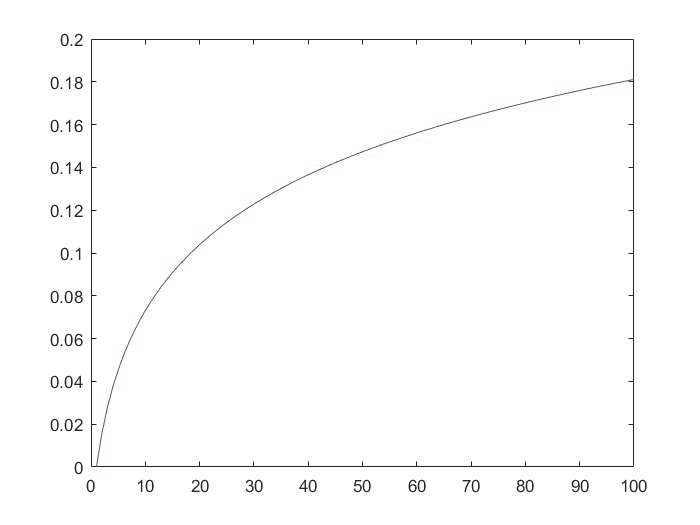
\includegraphics[height=8cm]{images/exchange-discount.png}

\caption{$MTC$ token deposit rank and cost for discount}
\label{fig:discount}

\end{figurehere}
\end{center}


\subsection{Fraud and Attack Protection}

\subsubsection{Exchange Covered Interest Arbitrage}

MTTP is trying create a fair ecosystem and find a balance between customers and exchanges. Firstly,  we will explain how exchange could archive a zero risk covered interest arbitrage.

Assume there are two orders $O_{a\rightarrow b}$, $O_{b\rightarrow a}$, form a loop, $r_{a\rightarrow b} \cdot r_{b\rightarrow a} > 1$. Exchange can input three new orders between those two. $O_{b\rightarrow c}$, $O_{c\rightarrow d}$, $O_{d\rightarrow b}$, to create a five orders-loop,  $r_{a\rightarrow b} \cdot r_{b\rightarrow c} \cdot r_{c\rightarrow d}\cdot r_{d\rightarrow b}\cdot r_{b\rightarrow a} = 1$. Exchange could make all the possible cost down to zero, once the transaction completed, it's like zero risk covered interest arbitrage
and $O_{b\rightarrow c}\rightarrow O_{c\rightarrow d}\rightarrow O_{d\rightarrow b}$. In order to stop those matter, MTTP requires: {\bfseries a verified loop cannot create more sub-loop to continue trading}.

\subsubsection{Denial-of-Service}

MTTP allows exchanges to selectively handle orders. Exchange can set up their own criteria and may choose to hide or reveal these criteria. Therefor MTTP does not see denial of service as a form of unethical behaviors.

\subsubsection{Massive Tiny Order Attack}
User can send out a large amount of tiny orders to attach exchanges. Exchanges, however, will reject most of these tiny orders because they do not yield satisfying profit when matched. As denial-of-service is not deemed as a form of attack, massive tiny order attack is not feasible.

\subsubsection{Insufficient Balance}

Malicious users may sign and spread out orders whose value inside the order is not zero but whose address actually has zero balance. This again is a not a good way of attack exchanges. Because exchanges will monitor and notice that some order's actual balance is zero and update these order's states accordingly then discard them.  

Exchanges do have to spend time to update order status, but can also choose to minimize these effort by, for example, blacklist some addresses and drop all related orders.

\subsubsection{Ring Filch}

A dodgy exchange could monitor all unconfirmed Match-Rings and broadcast the same rings with their own digital signature. We call this Ring Filch. In order to prevent Ring Filch, MTTP allows exchanges to use two steps in order to submit the order: 
\begin{itemize}
  \item Submit the hash of a Match-Ring, wait for confirmation.
  \item Submit the ring itself.
\end{itemize}
Hash rate:
$$h = H(r,  nonce)\text{, }$$
where $H()$ is a one-way hash function, $r$ is Match-Ring record. Hash Hash function contains a random number $nonce$.

\subsection{Market Depth\label{sec: marketdepth}}

Exchange no need to offer market depth data. Under this ecosystem,  both single organization and corporation can possibly pool all the unclosed orders into one market depth data. We can find out trading data between any two ERC20 tokens according to the agreement in chapter 3.3.

\subsection{Data Structure\label{sec: dataformat}}

All the orders can be represented by using one data structure due to adopting OTC module. This  data structure contains both digital signature and all parameters. Before the signature,  connect the parameter data from the orders into a set of data,  calculate the order's hash by using Keccak SHA3 method,  then sign by using this account's private keys with ECDSA.


\begin{verbatim}
message Order {
 address protocol;
 address owner;
 address outToken;
 address inToken;
 uint256 outAmount;
 uint256 inAmount;
 unit256 expiration
 unit256 fee;
 uint8 savingShare;
 bytes signature;
}
\end{verbatim}

Though there's no indicated price from the order, we are still able to find out through the formula: $outAmount / inAmount$ to get exchange rate $r$. All the actual exchange rate must be less than $r$. A user-friendly exchange should allow user to input $outAmount$, $inAmount$,  selling and asking price and use any two of those numbers in order to calculate the missing $outAmount$ or $outAmount$ figure.

Actual orders can be defined in two different ways: Definition A - transaction can be completed once number of token sold reaches $outAmount$ ; Definition B - transaction can be completed once number of token purchased reaches $inAmount$; Therefore,  we can setup a quote for exchange and mix-matching contract to help to define the trade. At our initial version,  we would support Definition A only.

Exchange could create a Match-Ring by using this data structure:
\begin{verbatim}
message MatchRing {
  Order[] orders;
  address feeRecipient;
  unit256 additionalDiscount;
  bytes signature;
  unit256 nounce;
}
\end{verbatim}


\subsection{Order Status\label{sec: orderstate}}


Order cannot be modified since it's been signed and announced. Data will be updated on the blockchain once smart contract find the matched order. Thus $inAmount$ and $outAmount$ will modified in corresponding with updated price. If $inAmount / outAmount$ shows 0,  it means the order has been fully closed. For example,  if the user wants to cancel the order,  a special request will be filed,  $inAmount / outAmount$ will be 0 to close the order. An expired order will not be updated on the blockchain - it can be tracked through the final cutting time. Hence,  we expect most of the orders will be expired or invalided.

\subsection{Smart Contracts\label{sec: contracts}}

MTTP consists of many smart contracts,  including:

\begin{itemize}
 \item \textbf{Mix-Matched Contract} is responsible for ensuring each order status in the loop,  calculating the price and volume,  transferring and interaction with other smart contracts,  API for MTTP;
 \item  \textbf{Order Contract} updates order database and support cancelling policy;
 \item \textbf{Registration Contract} maintains and upgrades service for exchanges who accepted MTTP,  support the token deposit from exchange and defaulted parameters backup;
 \item \textbf{Stats Contact} calculates the exchange volume and price between two tokens.

\end{itemize}

\begin{comment}
\subsection{支持ENS\label{sec: registration}}

\end{comment}

\section{Protocol Token \label{sec: protocoltoken}}


We will issue a token base on ERC20 Ethereum Token Standard called $MTC$ (displays in italics).


\subsection{Token Application}

$MTC$ will be use in the following areas:

\begin{itemize}
 \item \textbf{Gas Fees} --- $MTC$ can be paid as transaction fee for exchange. It will be simple and productive for the exchange to calculate all the cost in $MTC$. Same as request sender and receiver. We have mention this from previous chapter\ref{sec: fee}.
 \item \textbf{Deposit for Exchange Registration} ---Decentralized exchange mechanism has no limits on location or time. Thus,  those high turnover exchange would receive more orders and get more users. Hence,  we have setup a policy for those exchange that allow them to use $MTC$ to deposit into smart contract in order to increase exchange's credibility. Moreover,  it can also protect user from certain circumstance.
\end{itemize}

\subsection{Decentralized Governance}
Regulation has been updated as well as exchange's mechanism. Any $MTC$ holders have the voting power $S$, and number of the pledging $N$ and pledging time $CoinAge$
$$S = f(N,  CoinAge)\text{, }$$
where $CoinAge = H_{c}-H_{s}$. Joining CoinAge is to protect customers from speculations.

Decentralized mechanism include token registration, exchange registration, stat hash, deposit scale, maximum length, discount hash, subcontract address.
 \begin{itemize}
   \item \textbf{token registration} MTTP would adjust token,  low trading volume will be eliminated and new popular token will be replaced. however all the adjustment have to be recorded on smart contract.
  \item \textbf{exchange registration} Only those exchanges accept MTTP would allow to start trading.
   \item \textbf{stat hash} Data will increase to certain amount after a long period operating. The more data exchanges have,  the more accurate system computation ability has.
  \item \textbf{deposit scale} Deposit for each exchange should be measurable. if the amount is huge,  the liquidation gets worse; verse vice.
   \item \textbf{maximum length} Technically, more orders can create more profit,  however the risk of failure also increase. As well as the trading cost.
   \item \textbf{discount hash} Discount hash will be adjust with the market. Below figure shows, blue line represents normal market, yellow line represents supply market, red line represents demand market.
\begin{center}
\begin{figurehere}
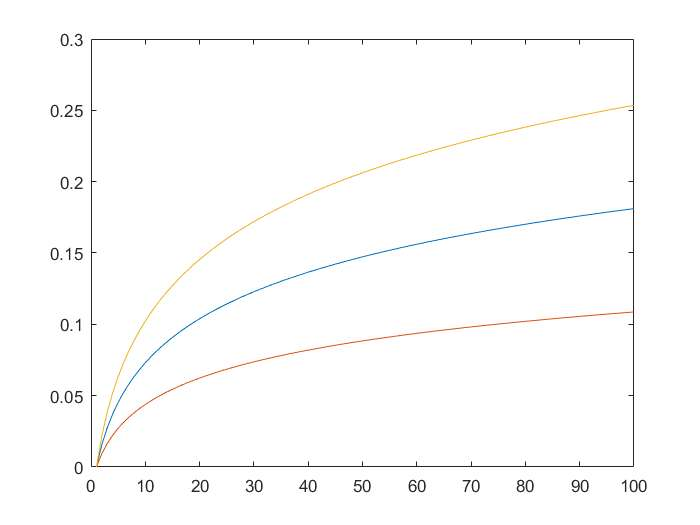
\includegraphics[height=10cm]{images/rate_adjust.jpg}
\caption{discount rate after adjustment}
\label{fig: dischargeRateAdjust}
\end{figurehere}
\end{center}

   \item \textbf{subcontract address} If MTTP exchange based on Ethereum ecosystem,  then smart contract cannot be modified. Therefore,  update MTTP's subcontract in order to modify subcontract address.
 \end{itemize}

%\footnotemark

\subsection{Token's Liquidability}

MTTP's token is based on ERC20 Ethereum Token Standard and it can be liquidated through MTTP smart contract. It means MTC trading can be made out of centralized exchange. All the ERC20 Ethereum tokens can be exchanged to MTC token( assume pre-order is MTC,  with zero fee) by adopting MTTP's decentralized mechanism.


\section{Exchange\label{sec: exchange}}

Exchange is unable to guarantee all the transaction could make profit after adopted MTTP. First reason is high operating cost. Secondly,  high expectation cannot match the actual outcome. There are few other reasons would cause this saturation. Overall,  both exchange platform and other parties have reciprocal relationship: exchange looks for profitable order; while order senders look for exchange with lowest fee.
Exchange is not responsible for users ERC20 token after accepting MTTP. The workload has moved from money deposit,  withdrawal,  internal virtual account management to mix-matched order service. Meanwhile,  for the users,  MTTP does not require customer to deposit or lock any asset, that means asset have zero risk to get stolen, at same time single order can mix and match multiple trades.
For Non ERC20 asset,  exchange can offer asset tokenization service.

\subsection{Regular and MTTP Exchange Comparison}
In a regular exchange,  "Maker" send a order and "Taker" receive order. The exchange price highly depends on sender's end. Under MTTP circumstance,  it has adopted Over-The-Counter (OTC) module.
In current market,  there is considerably high risk for users to trade in those platform,  no law to regulate the exchange if they vanish. But with MTTP,  users do not to deposit money to the exchange anymore. All the transactions will be made among users coin address.
Another feature for MTTP is that it has change the "Trading Pair"concept. Transaction can be completed with multiple parties instead of 2 parties in current exchange.


\begin{table}[hbt]
  \centering
\begin{tabular}{p{5cm}|p{2.5cm}|p{2.5cm}} %设置了每一列的宽度,强制转换。
&Centralized Exchange & MTTP Exchange \\ %用&来分隔单元格的内容 \\表示进入下一行
    \hline
Deposit for the order& Yes & No \tablefootnote{Exchanges execute under MTTP ecosystem do not require any deposit - Tokens are kept in user's wallet, no transaction will be made before the full contract close. As a result, no account stolen or asset lost risk.}\\
\hline
Frozen Account& Yes & No \tablefootnote{MTTP exchanges do not require freeze trading fund --- If user partially or fully modify the fund, the contract will be withdraw automatically.}\\
\hline
Deposit/Withdraw& Yes & No \tablefootnote{Sender's order can be distributed to multiple receivers partially or fully take under MTTP ecosystem.}\\
\hline

Internal Trading Risk& Yes & No\tablefootnote{All matching trades are based on smart contract on blockchain, data are immutable and transparent.}\\
\hline
Customer loss from exchange closing& Yes & No\tablefootnote{ MTTP exchanges are not responsible for tokenization, thus MTTP users will not be affected if exchanges wind up. For example, if blockchain account will not affected if the mining terminated. In conclusion, Exchanges are responsible for matching trades. Smart contract will complete clearing and settlement. Therefore, assets are always kept in user’s blockchain account.}\\
\hline
Transaction is the main income& Yes & No\tablefootnote{Transaction fee is not a mainstream income for MTTP exchanges, mainstream comes from “profit of transaction cost saving”, because it can effectively encourage trade matching.}\\
\hline
Accept Legal Currency& Yes & Yes\tablefootnote{MTTP exchanges fully support asset tokenization, hence, it requires legitmate currency being tokenized on ERC20 standard.}\\
\hline
Can be traded among multiple exchanges& No & Yes \tablefootnote{MTTP allows multiple MTTP exchanges partially or fully trade off one order at same time.}\\
\hline
Fairness for Maker and Taker& No & Yes \tablefootnote{Transaction price is closed to the balance price instead of being tend to maker’s offer price under MTTP protocol.}\\
\hline
Mix and Match Trading& No & Yes\tablefootnote{ MTTP exchanges’ multiple supporting feature can help sender to find the most profitable order.}\\
\hline
Supervision & Strong & Weak\tablefootnote{MTTP exchanges do not require deposit, Clearing and settlement are made through open source smart contract. Hence, regulation is not necessarily if there's no asset tokenization occurred.}\\

  \end{tabular}

\caption{Contrast between centralized exchange and MTTP exchange} %显示表格的标题
\end{table}

%\footnotemark


\section{Summary\label{sec: summary}}

We describe a protocol that facilitates decentralized exchange of ERC20 tokens on the Ethereum blockchain. MTTP allows multi-token transaction exchange,  as well as it accepts exchange liquidation on blockchain; This whitepaper has explained how the mechanism work under different circumstance. In additional,  the benefit that MTTP has brought to current exchange mechanism.
MTTP protocol fits any ERC20 and smart contract blockchain platform. After many discussion,  our team will develop MTTP on the Ethereum blockchain.
We also plan to create a non profit foundation for MTTP through crowdsale and issuing ICO.

\section{Acknowledgements\label{sec: acknowledgement}}

We would like to express our gratitude to our mentors,  advisers and to the many people in the community that have been so welcoming and generous with their knowledge. In particular,  we would like to thank Xing,  Jiang; Xiaochuan Wu; Zhen, Wang and Jun, Ma for reviewing and providing feedback on this work. We are also welcoming more feedback from community.

\newpage  
\bibliography{whitepaper}
\bibliographystyle{unsrt}

%\newpage
%
%\begin{appendices}
%\section{$MTC$ Token Crowdsale\label{sec: ico}}
%
%We plan to issue 100 million MTC token,  8000 million tokens will be allocated to crowdsale participators. and rest 20 million tokens will be allocated to the foundation initiator for maintain and developing the community in the next 5 years.
%
%ICO will start pre-sale to investors and crowdsale in 2017 July. We plan to raise XXXX ETH
%Initial spending plan;
%
%\begin{table}[hbt]
% \centering
% \begin{tabular}{l|c}
%   Purpose    & Percentage\\
%  \hline
% Tech Development  & 50\% \\
% Community Building & 20\% \\
% Marketing     & 15\% \\
% Legal and Law   & 15\% \\
% \end{tabular}
% \caption{ Plan for token expense}
%\end{table}
%
%
%
%Project ICO and Timetable
%\begin{table}[hbt]
% \centering
% \begin{tabular}{l|l}
%Time  & Target\\
%  \hline
% 2017/06 & Whitepaper release, Project start-off \\
% 2017/07 & Module Development Completion \\
% 2017/08 & MTTP open source committee(Foundation)set and Pre ICO closed \\
% 2017/08 & ICO schedule \\
% 2017/09 & ICO start \\
% 2017/10 & ICO close and release result \\
% 2017/11 & $MTC$Token IOU launch at exchange \\
% 2017/12 & Test $MTC$ token on ETH \\
% 2018/02 & Commencement \\
% 2018/04 & Issue $MTC$ token on ETC \\
% \end{tabular}
% \caption{Project Schedule}
%\end{table}
%
%\subsection{ETH/ETC Due-chain issue\label{sec: chains}}
%
%Though we only accept ETH as our ICO token,  but we also consider ETC token's potential on developing smart contract. Hence,  we will issue our token $MTC$ on both Ethereum (ETH)and Ethereum Classic(ETC).
%
%
%\subsection{Risk Awareness\label{sec: risks}}
%
%Initial crypto-token offering (ICO) now is a popular way for crowdsale,  it contains certain risks. Participators should be fully aware of all the potential risk and The MTTP Foundation hereby expressly disclaims its liability,  and shall in no case be liable to any person,  for: 
%\begin{itemize}
% \item any person's participation in the Campaign in violation of any anti-money laundering,  counter-terrorism financing or other regulatory requirements that are imposed in any jurisdiction;
% \item any person's participation in the Campaign in violation of any representation, warranty,  obligation,  covenant or other provision under this Prospectus,  and the resulting failure or inability to retrieve his/her payment or to claim relevant purchased $MTC$ for Crowdsale;
% \item early termination of the Campaign for any reason;
% \item failure or abortion of the Quantum development and resulting failure to deliver the purchased $MTC$ for Crowdsale to the Purchasers;
% \item any risk factors disclosed in this Prospectus and any damage,  loss, claim, liability, punishment, cost or other adverse impact that is caused by, associated with, in connection with, incidental to or consequential to that risk factor.
% \item if there is any separate agreement between a Purchaser and a Crowdsale Intermediary,  this Prospectus shall take precedence over that agreement in all respects. The MTTP Foundation shall in no case be bound by,  and hereby disclaims any liability under,  the foregoing agreement.;
% \item failure or abortion of the MTTP development and resulting failure to deliver the purchased $MTC$ for crowdsale to the Purchasers;
%
%\end{itemize}
%
%
%
%\end{appendices}
\end{document}
